\documentclass{picocon-fanzine}
\usepackage{xcolor}
\usepackage{soul}
\usepackage{array}
\usepackage{textgreek}
\usepackage{pgfplots}
\usepackage{pgfplotstable}
\usepackage{xcolor}
\usepackage{soul}
\usepackage{amsmath}

\renewcommand{\tombstone}{%
  
\includegraphics[height=\fontcharht\font`\B,clip]{img/tombstone}%
}

\begin{document}
\thispagestyle{empty}
\vspace*{8cm}
\begin{center}
\texttt{\textbf{\Large PICOCON 40}}
\end{center}
\begin{center}

\includegraphics[width=1\textwidth]{img/twisted-poster.jpeg}
\end{center}
\begin{center}
\texttt{\textbf{\Large FANZINE}}
\begin{center}

\includegraphics[height=0.1\textwidth]{img/black-rose.jpg}
\end{center}
\end{center}
\clearpage
\setcounter{page}{1}
\head{From the Editors}

Hello there! welcome to our humble little fanzine! 

Contained within these 30 hallowed pages are a collection of twisted and fantastical stories and art sent to us by current students, committee, and anyone else who felt compelled to make something for us to display.

We're pleased to finally have another fanzine, after last year where got only 1 submission, and so sadly had to forgo running this fanzine. So relax, and enjoy some twisted stories.
\tombstone

%\hfill \parbox{0.5\textwidth}{{\large\textbf{Jean Lo}}\\Wyrmtongue
%  Editor}
\hfill \parbox{0.5\textwidth}{{\large\textbf{\textemdash{} Luke Conmy - \st{Treasurer} \st{The one responsible for the Homestuck bullshit} Unofficial Editor}}\\\hspace*{1.7em}March 2023}
\vfill

Thank you, Luke (also hi new editor here), and we return all the love to those who sent us their wonderfully twisty work to this fanzine. For those of you who've been handed this humble collection, be sure to check out the Picocon \emph{Wyrmtongue} to find out what's happening, and most of all, enjoy the convention!
\tombstone

\hfill \parbox{0.5\textwidth}{{\large\textbf{\textemdash{} Clifford Chan - The other (very experienced) Editor}}\\\hspace*{1.7em}March 2023}
\vfill

\tableofcontents
\vfill

\clearpage
\story{Rumpelstiltskin}{Rebecca Allday}{A twisted retelling of a classic fairytale}{txt/rebecca-a}
\vspace{50px}

\begin{center}
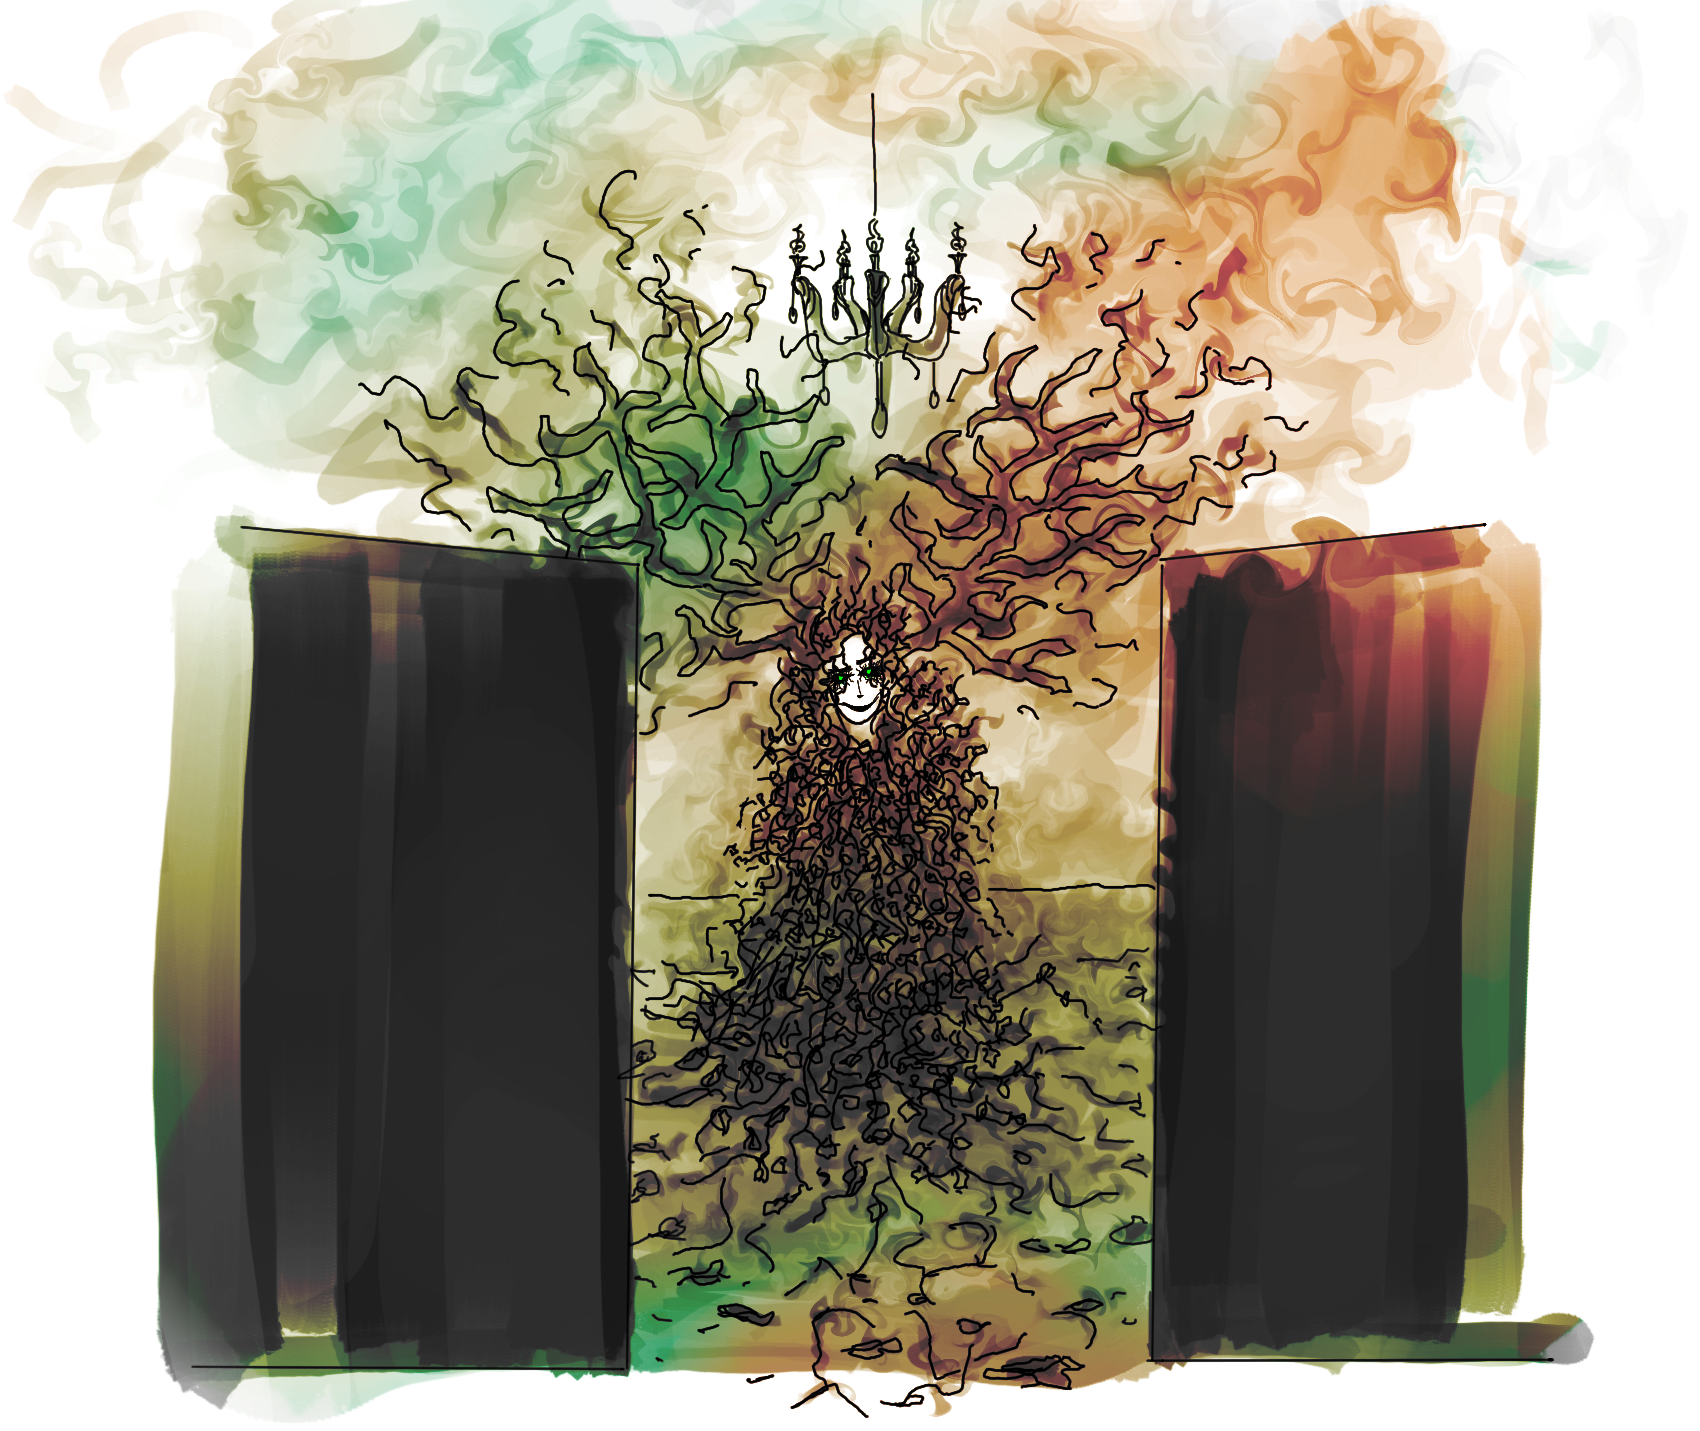
\includegraphics[width=1\textwidth]{img/rumplestiltskin.png}
\end{center}

\centerline{\emph{Illustration by Rebecca Allday}}
\vfill

\clearpage
\story{Seeing the Trees}{Luke Conmy}{What if I just left, what would I have to lose?}{txt/luke-c}
\vfill

\clearpage
\story{The View from the Light-spire}{Sophie Reck Pointon}{A world of belief swept away by mist}{txt/sophie-r-1}
\vfill

\clearpage
\story{Slaughterhouse}{Clifford Chan}{Dark secrets are uncovered in Mr Edgars' home...}{txt/cliff}
\vfill

\clearpage
\artpage{Twisted Paths}{Irene Soto}{img/Irene_A2Mod2}
\centerline{\emph{Inspired by Dimension 20 \textendash{} Neverafter campaign  \tombstone}}
\vfill

\clearpage
\story{My Immortal (Dalek style)}{Sophie Appleyard}{My Immortal fanfiction but with more Daleks}{txt/sophie-a}
\vfill

\clearpage
\story{Surreal}{Anand Doshi}{A short supernatural suspense}{txt/anand-d}
\vfill

\clearpage
\story{Fairy-Phone}{Juairiyah Raqib}{Fairytale villainesses have their own problems}{txt/juairiyah-r}
\vfill

\clearpage
\story{The Room-Where-the-Aurora-Looks-In}{Sophie Reck Pointon}{Involving a Sorcerer, a Princess and some morally ambiguous magic}{txt/sophie-r-2}

\clearpage

\clearpage


\clearpage


\clearpage
\thispagestyle{empty}
\vspace*{\fill}
\begin{center}
  
\includegraphics[width=0.5\textwidth]{img/icsf-logo}
\end{center}
\vspace{4em}

\end{document}
